\section{Introduction}



Additive manufacturing (or 3D Printing) is an emerging technology, in which
different objects are printed in layers having a 3D model as a reference. This technology made rapid prototyping faster and enabled the creation of custom-shaped objects. However this process is not always perfect and printing errors are to be expected. Manually reviewing every print job is a tedious labor work and naturally the desire of automatization of anomaly detection rose. \\
One interesting 3D printing technique, sand 3D printing, stands out by not using any heat. This allows printing objects of very large sizes, but comes with a specific type of printing defects: scratches. \\
In this thesis a YOLO-based neural network solution is proposed and analyzed for this automatization procedure. \\
TODO: motivation
TODO: one abstraction layer above

TODO: insert example of scratch


\subsection{Printing process}
The 3D printer in the experiments at hand is sand based, more specifically binder jetting technology. With this technology, a layer is printed by laying a powder bed, then the printer applies drops of binding agent in regions of the bed to bond the powder particles together \cite{binder_jetting}. For each layer a bitmask is provided, which shows the regions that need to be printed. \\
In order to better track the printing process, the 3D printer has an internal camera that captures each printed layer. The captured images are then calibrated. In figure \ref{fig:layer_bitmask} a printed layer and the respective bitmask can be seen.\\
In our case the printing errors are scratches on the printed surfaces like in figure \ref{fig:layer_00325_marked_cropped}. \\

TODO insert figure here
% \begin{figure}[ht]
%   \centering
%
%   \begin{subfigure}{\textwidth}
%     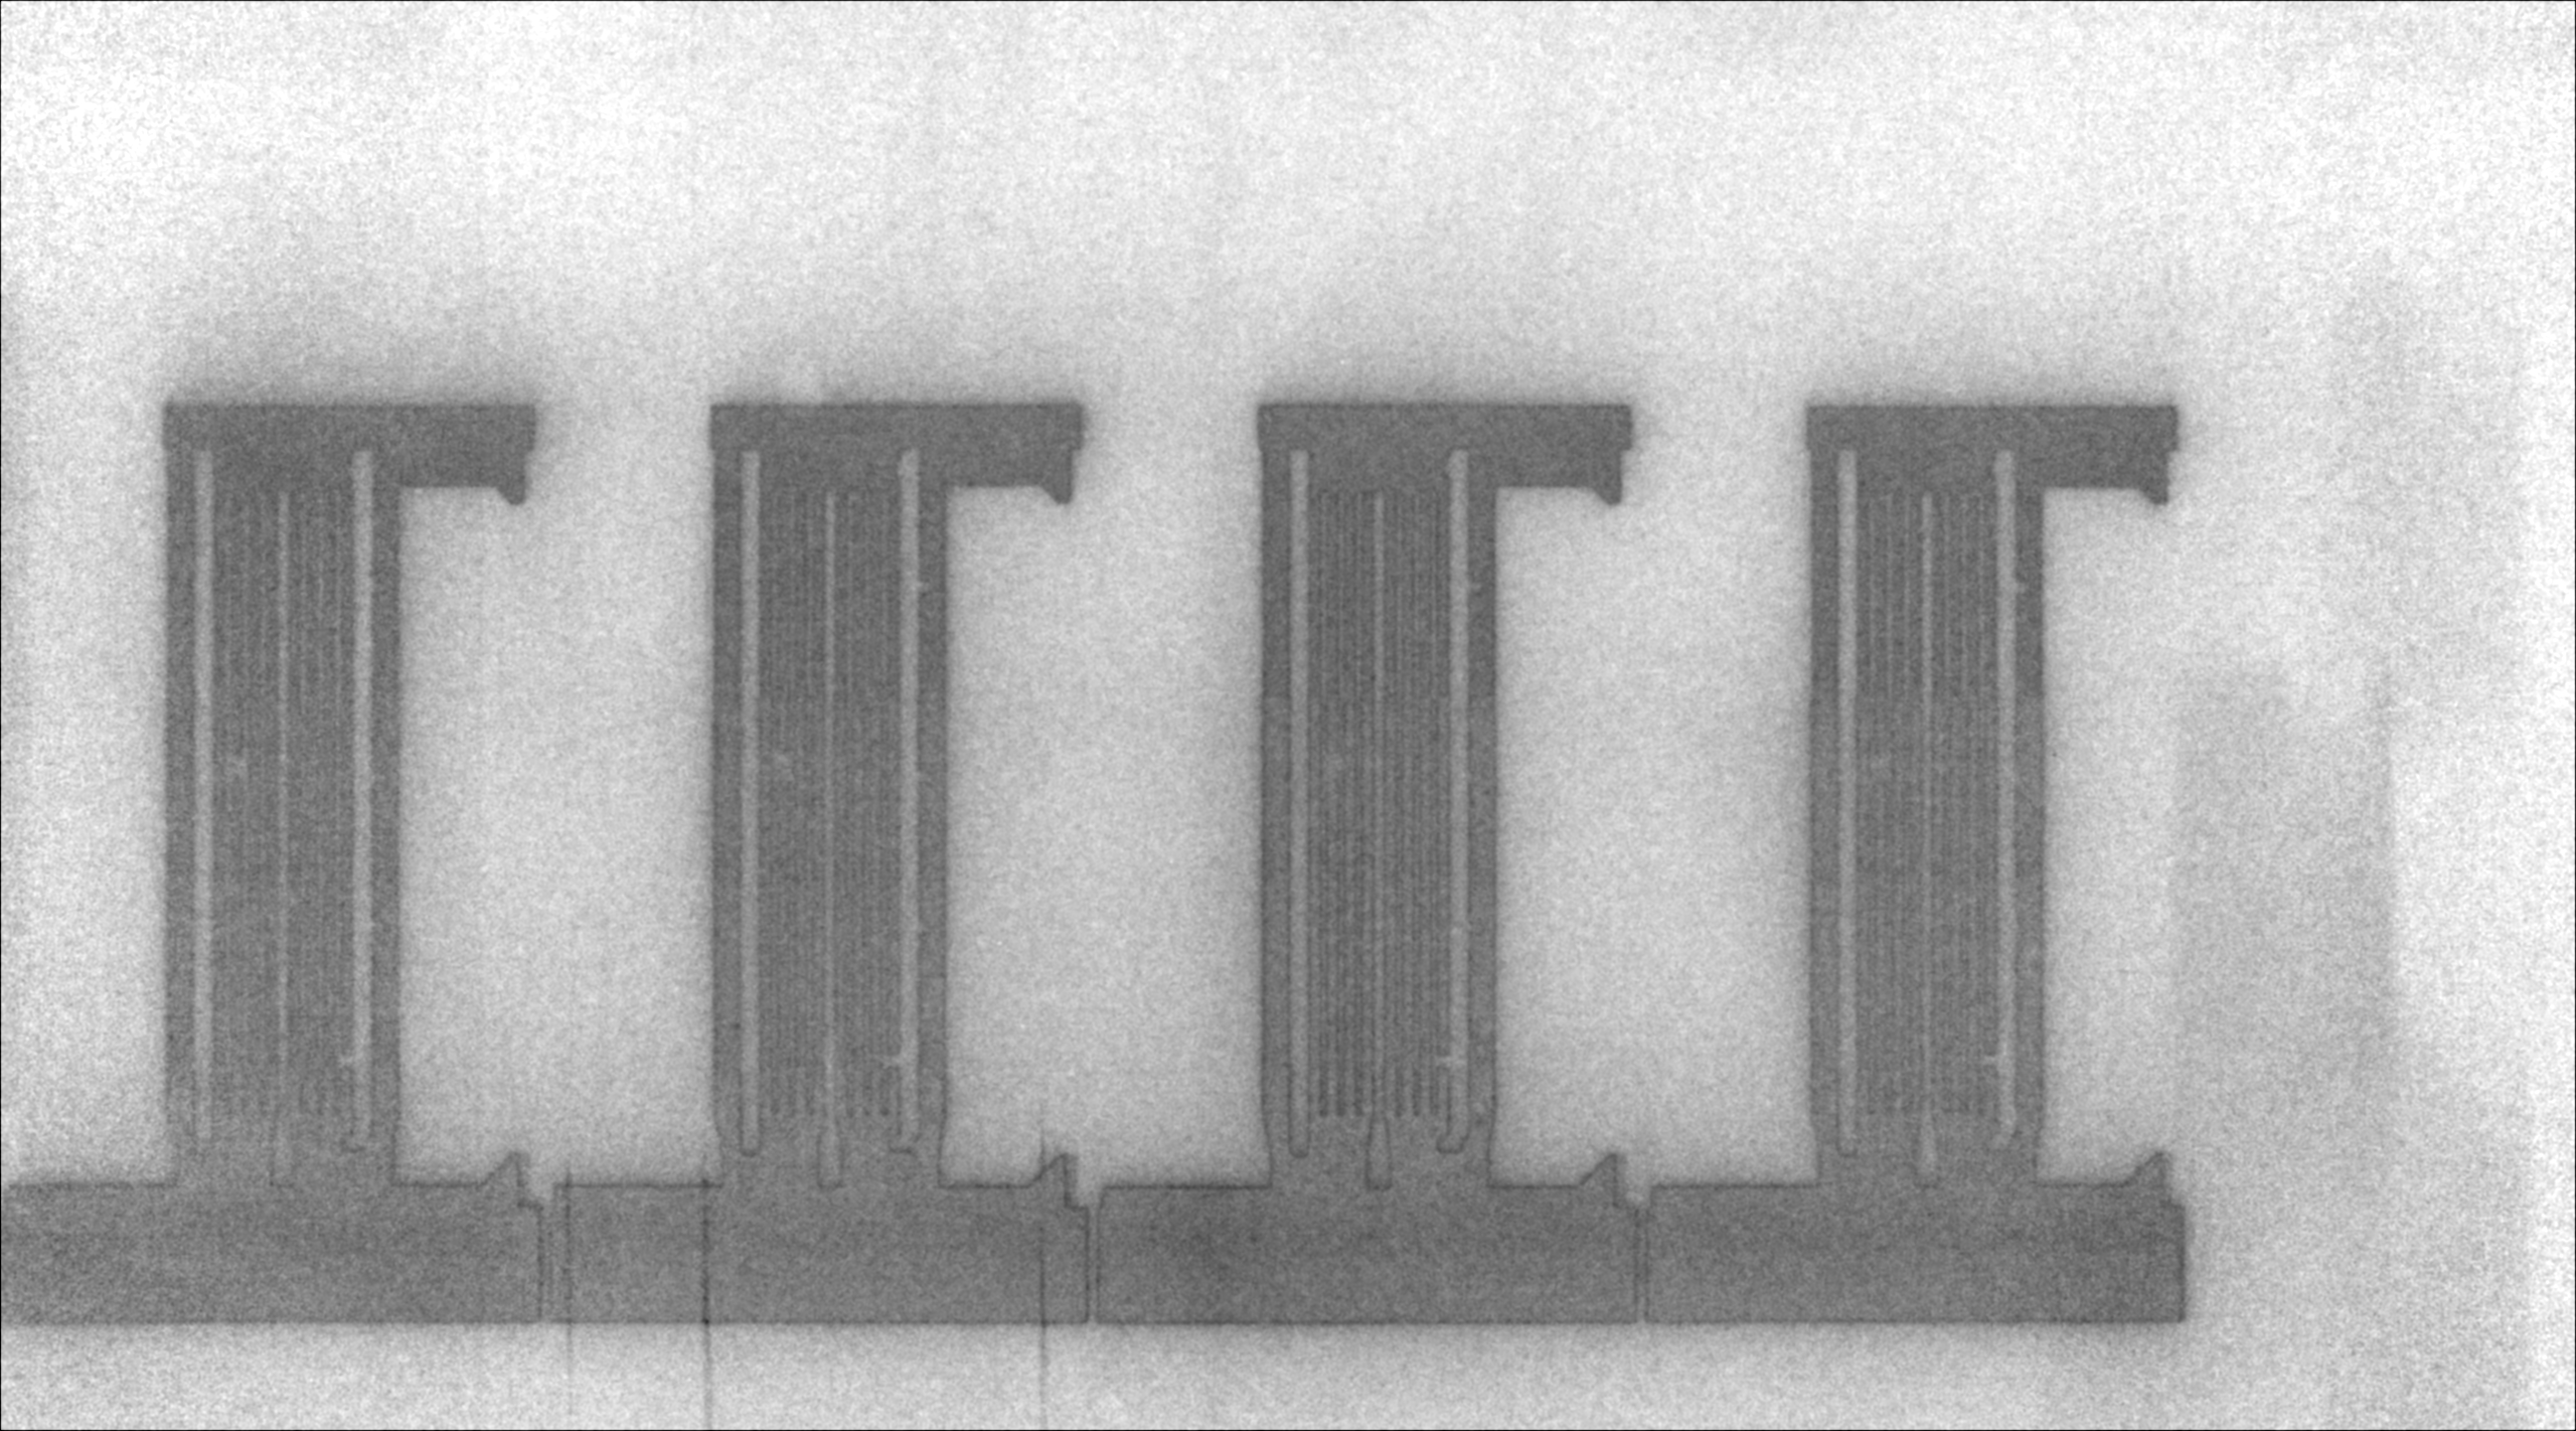
\includegraphics[width=\textwidth]{images/layer_00325}
%     \caption{Calibrated capture of a layer.}
%     \label{fig:layer}
%   \end{subfigure}
%
%   \begin{subfigure}{\textwidth}
%     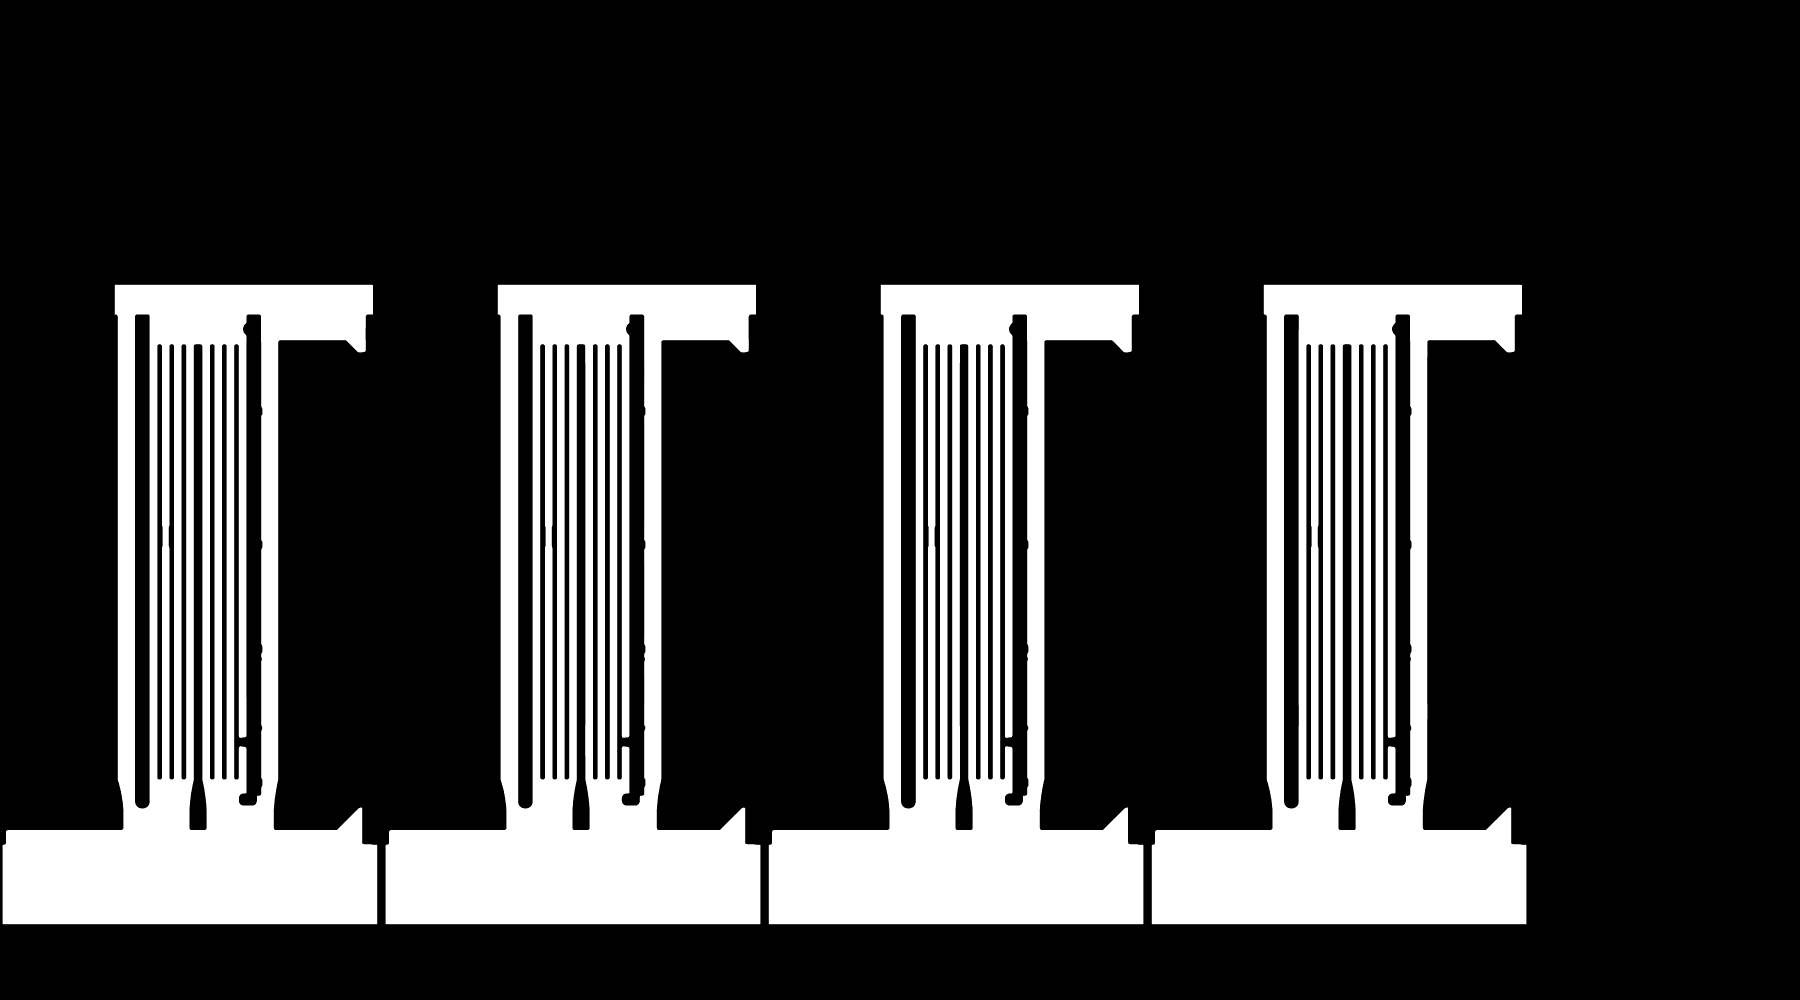
\includegraphics[width=\textwidth]{images/bitmask_00325}
%     \caption{Bitmask used by 3D Printer as layer model.}
%   \end{subfigure}
%
%   \caption{Printed layer with the respective bitmask.}
%   \label{fig:layer_bitmask}
%
% \end{figure}


\begin{figure}[ht]
  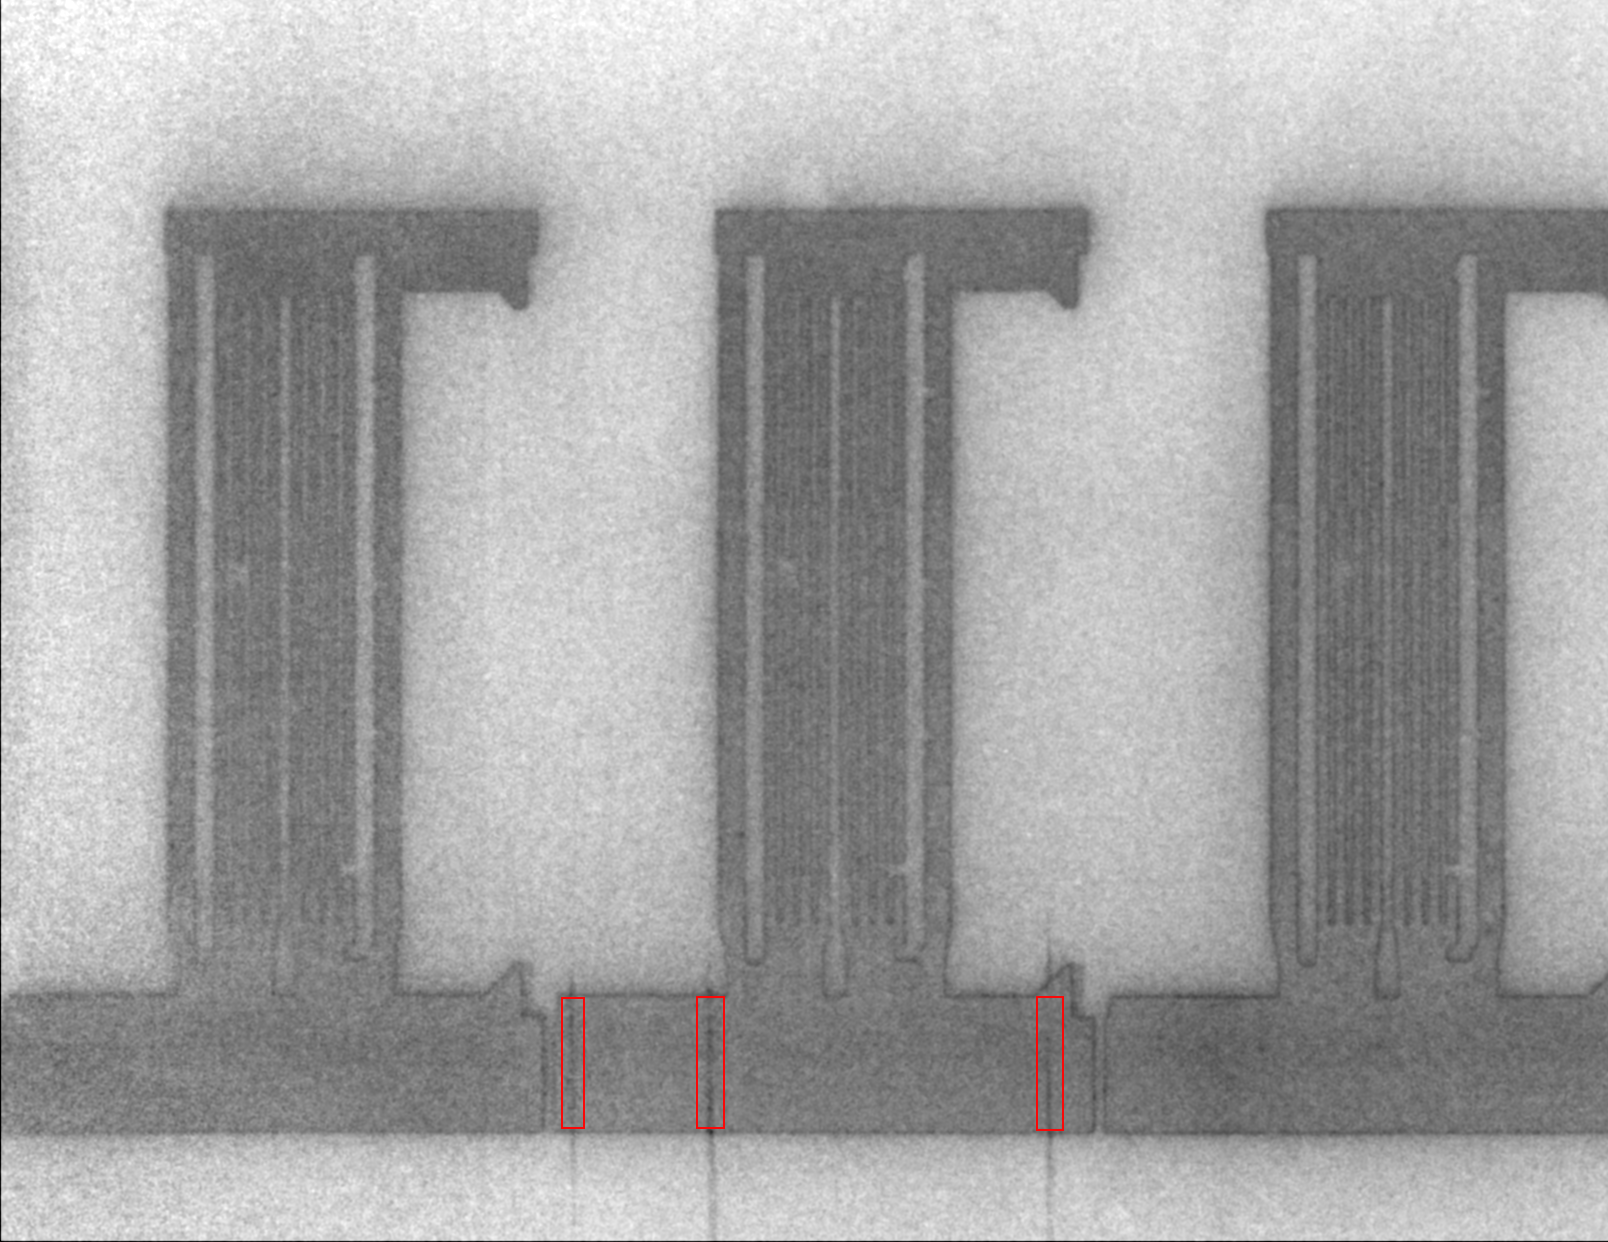
\includegraphics[width=0.65\textwidth]{images/layer_00325_marked_cropped}
  \centering
  \caption{Scratches marked from figure \ref{fig:layer}}
  \label{fig:layer_00325_marked_cropped}
\end{figure}

TODO: OD with NN, bb and semantic segmentation, vezi bookmark nou
\subsection{Object Detection (With Neural Networks)}
There are a variety of techniques used to perform object detection. Initially, object detection was posed as a non-neural computer vision problem, but this required a constant and tedious manual tuning of parameters. In order to avoid this tuning, feature-based machine learning algorithms were developed e.g. Viola-Jones algorithm \cite{viola_joines_paper}. In this way the parameter tuning was partially automatized, but it still required manual tuning like selecting the optimal Haar features for the Viola-Jones algorithm.
One step further in this direction was the introduction of deep-learning based methods, which use a neural network at heart. A trained neural network would be albe to detect objects with way less parameter tuning. The drawback is that a considerable amount of labeled data for training is now required, which mostly is manually labeled. Luckily, today there are many open source labeled datasets that easily contain hundreds of thounsands of images e.g. ImageNet Dataset \cite{imagenet_site}, OpenImages Dataset \cite{openimages_site}. \\
Because of the already labeled datasets, the manual labor for deep-learning based methods was greatly reduced and the focus shifted towards those kind of methods, leading to the creation of many innovative models. One distinction among deep-learning based methods, regarding data labeling, is that the objects can be labeled with bounding boxes or segmentation masks. Models that use bounding boxes tend to train and predict faster, while models with segmentation masks will have the benefit of optimizing predictions to a pixel level. Another consideration would be that, if manual labeling is required, drawing bounding boxes is easier and less error prone than drawing an outline for segmentation masks. \\

\begin{figure}[!h]
\centering
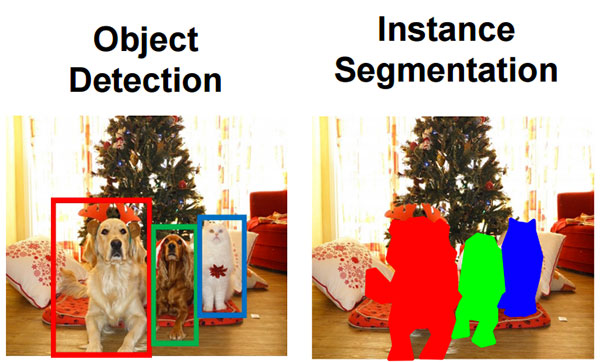
\includegraphics[width=0.65\textwidth]{images/bbs_vs_seg}
\caption{Labeling methods: on the left bounding boxes, on the right segmentation masks}
\end{figure}

Regarding the architecture of neural networks, the detection process may have one or two stages. In a single stage network the prediction is made directly from the extracted features of the image, while in a two stage network the network proposes some regions in the first stage and in the second stage the proposed regions are classified. Initially, single stage detectors predicted faster and could be used for real-time detections, but where performing poorer than two-stage detectors. Conversely, two-stage detectors were not optimal for real-time detection, but were more precise. This rule of thumb got overwritten with the release of You Only Look Once object detector (YOLO).

\begin{figure}[!h]
\centering
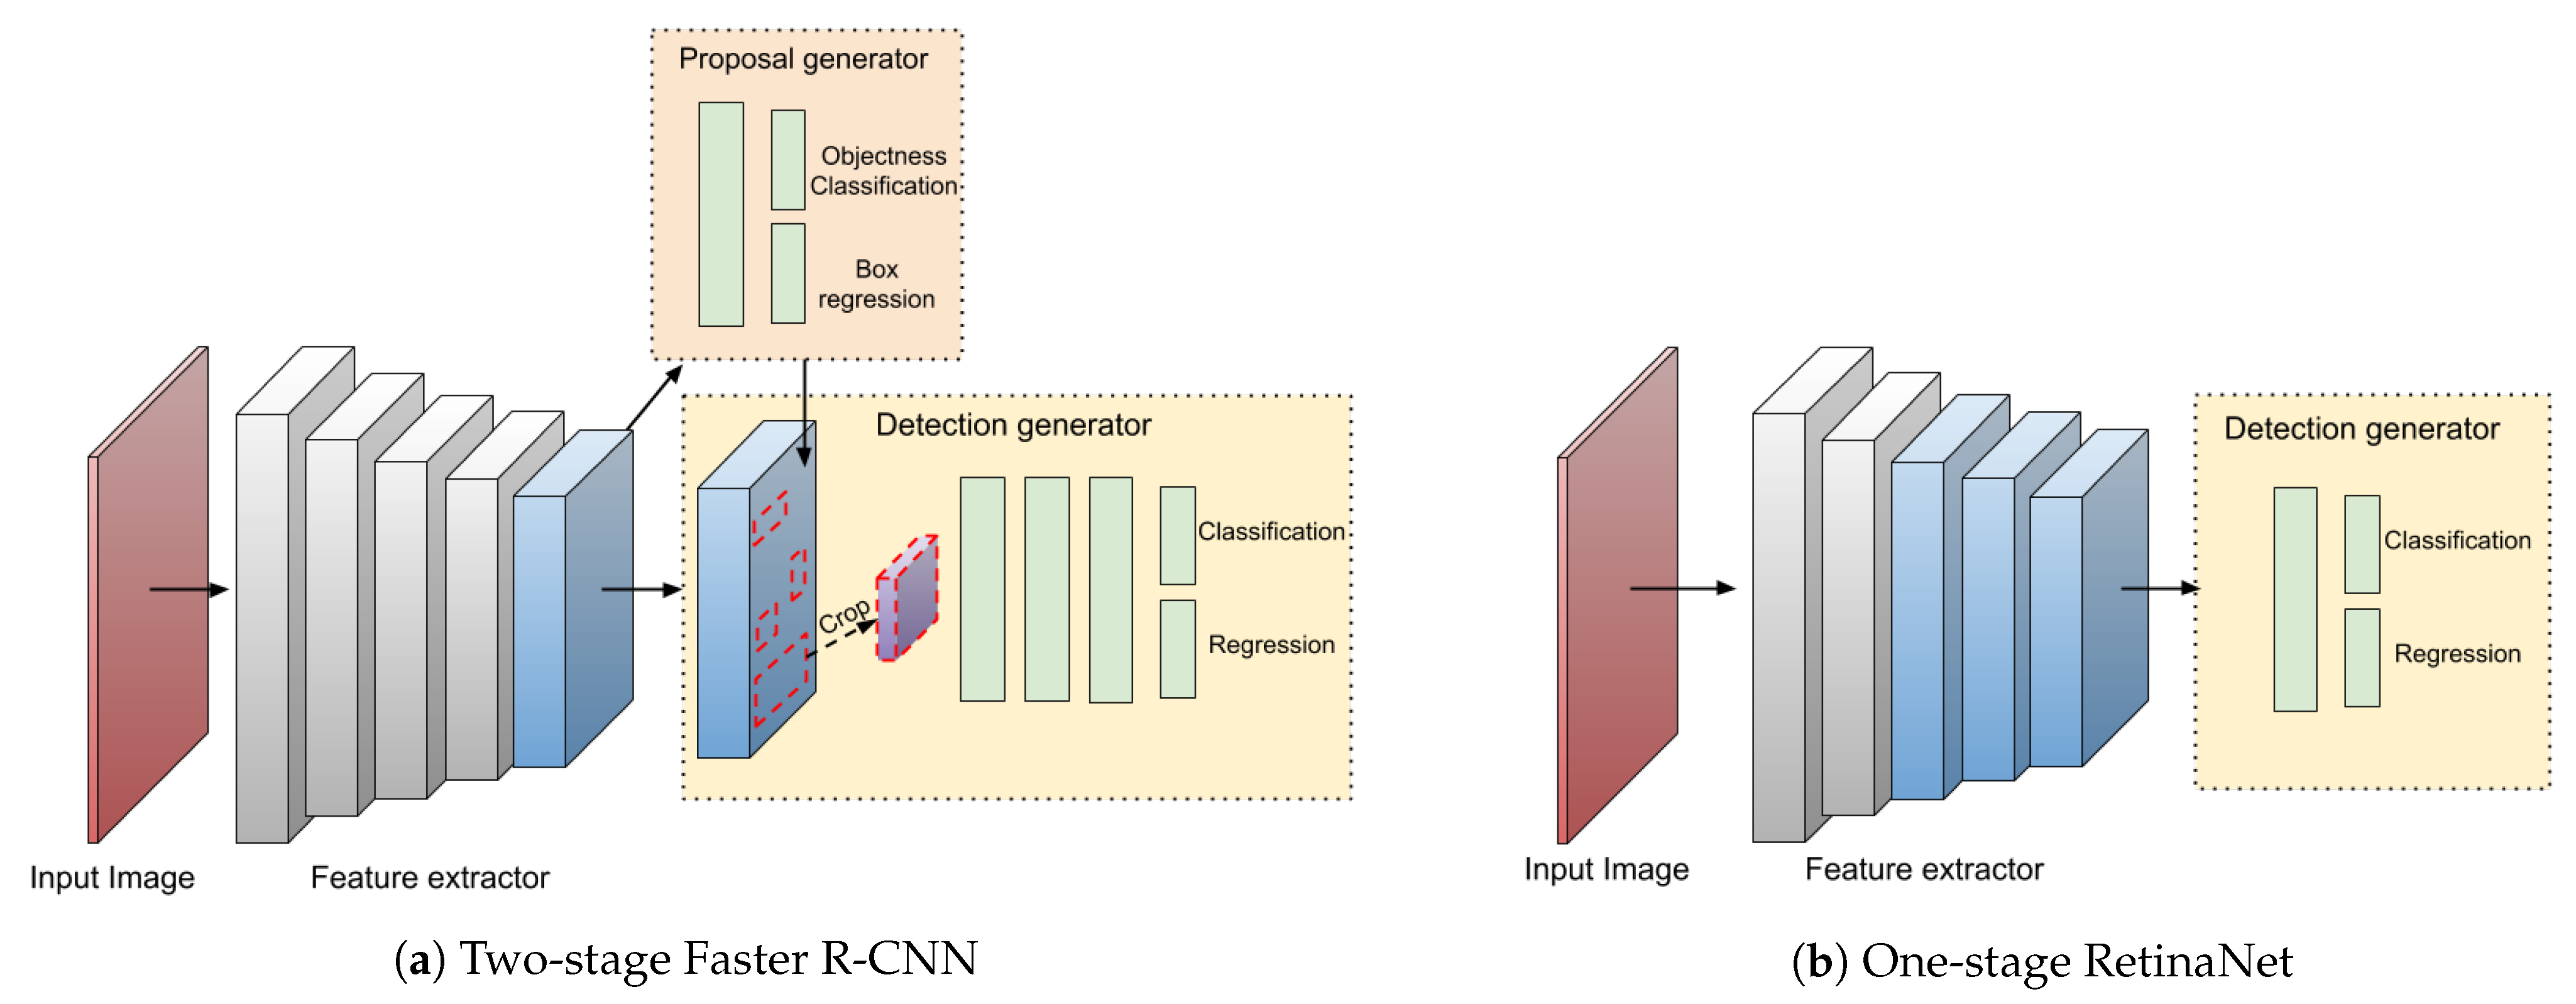
\includegraphics[width=0.75\textwidth]{images/single_stage_vs_two_stage}
\caption{Comparing stage types of object detectors.}
\end{figure}



The first YOLO object detector, now known as YOLOv1 \cite{yolov1_paper}, got a lot of attention for outperforming the then state-of-the-art object detectors such as DPM \cite{dpm_paper}, Fast R-CNN \cite{fast_rcnn_paper} and Faster R-CNN \cite{faster_rcnn_paper}. Also the simplicity of YOLO was quite refreshing for using only 24 convolutional layers and 2 fully connected layers only, unlike the sophisticated R-CNN based architectures. \\
Even if in some very deep model variations of Fast and Faster R-CNN the mean average precision (mAP) was slightly better,the FPS counter would take a massive hit e.g. 0.5 FPS only for Fast R-CNN. \\

\begin{figure}[!h]
  \centering
  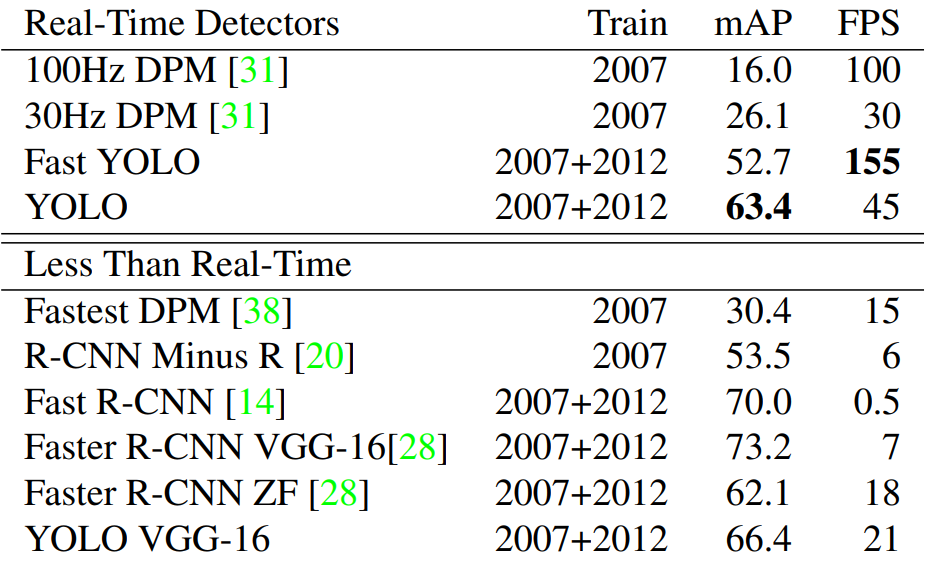
\includegraphics[width=0.75\linewidth]{images/yolo_images/compare_yolov1}
  \caption{TODO: make own table. YOLOv1 compared to then state-of-the-art models \cite{yolov1_paper}}
\end{figure}


This first successful initial release of YOLO was a launch pad for development of subsequent YOLO versions, so that a new class of object detectors was born. This class of architecture contains 3 main components: backbone, neck and head.
The backbone has the role to extract features from the image, while the neck tries to aggregate the features from different stages from the backbone. In the end the head does the prediction. Usually the backbone has a quite simple build like ResNet-101 and Darknet-53 \cite{yolov3_paper}.For feature aggregation SPP \cite{spp_paper} and FPN \cite{fpn_paper} are a popular choice . \\
Later on, different research groups developed their own YOLO-based object detectors and non-canonical versions like YOLOv5 \cite{yolov5_git} and YOLOR \cite{yolor_paper} were created. With this many releases from different research groups, simply taking the latest YOLO version was not a viable choice anymore and for this thesis multiple versions have been tests.\\

\subsection{Main Challenges} \label{intro:challenges}
In this section an overview of some ...

\textbf{Small dataset:}
As seen in section TODO, the images of the printed 3D layers are grayscale images and the target objects are some long thin scratches. This is in contrast with the open datasets that contain RGB images with 80 different objects, which do not even closely resemble a scratch. As a consequence, only the small dataset at hand of about 2300 images can be used for training. The situation gets even worse after discovering that only TODO images contain scratches. \\
A fortunate thing is that the scratches can fit very good in bounding boxes and no extra precision will be provided by the more tedious, time-consuming segmentation masks. This leads to the next point of labeling. \\

\textbf{Labeling the dataset: -> Id relevant scratches, consistency of the labels}
When labeling the dataset, it was discovered that some scratches might initially appear on a layer and then slowly fade away, as seen in figure TODO. In the middle of the fading process the scratch transitions into a dark gray spot and finally disappears. This makes the labeling difficult, since it is hard to tell in which exact layer a scratch transitions into a dark gray spot.
It is important to be consistent and have an objective evaluation of the scratches, but humans are not capable of this. This is similar to Sorites Paradox [TODO cite]. Therefore, a metric is needed to ensure consistency.\\


\textbf{Domain Knowledge Integration:}
As seen in figure TODO, two close edges might look like a scratch, but the bitmask can be used to clarify the situation. This exact process of comparing the layer image with the respective bitmask is the motivation of including also the bitmask for training and inference. The problem is that most models take exactly one image and a file with labels as input and now a bitmask needs to be included somehow.\\
Another problem is that small artifacts from previous layers can be visible in the current layer, which again might look like a scratch. This means that looking at previous bitmasks is also helpful during labeling. Therefore, the model needs to be aware also of previous bitmasks. Now the problem from the previous paragraph evolved into including multiple bitmasks. \\


\textbf{Choosing the neural network:}
Due to the large amount of modern neural networks, a calculated decision needed to me made. As presented in the previous section, YOLO models are currently showing a good mean average precision, despite using a single-stage approach. Another benefit of YOLO models is that the scratches can be precisely contained into a bounding box and there would be no benefit of using a model with segmentation masks. \\
There are currently a multitude of YOLO versions developed by different research groups. The final decision was to use YOLOv5 by ultralytics \cite{yolov5_git} since it quickly displayed a good performance, was written in a popular framework like PyTorch and provided support for logging and debugging tools. Other versions, such as YOLOv4 \cite{yolov4_paper}, YOLOX \cite{yolox_paper} and YOLOR \cite{yolor_paper}, were some interesting candidates, but each came with it's drawbacks. YOLOv4 had similar performance to YOLOv5, however it had longer training times and a very rudimentary logging system (no support for tools like Tensorboard). YOLOR and YOLOX had interesting twists regarding the architectures, but YOLOX used a custom framework called MegEngine \cite{megengine_git} and YOLOR lacked documentation and large community support. A few initial experiments were also not better than YOLOR or YOLOX. \\


\begin{figure}[ht]
  \centering

  \begin{subfigure}{\textwidth}
    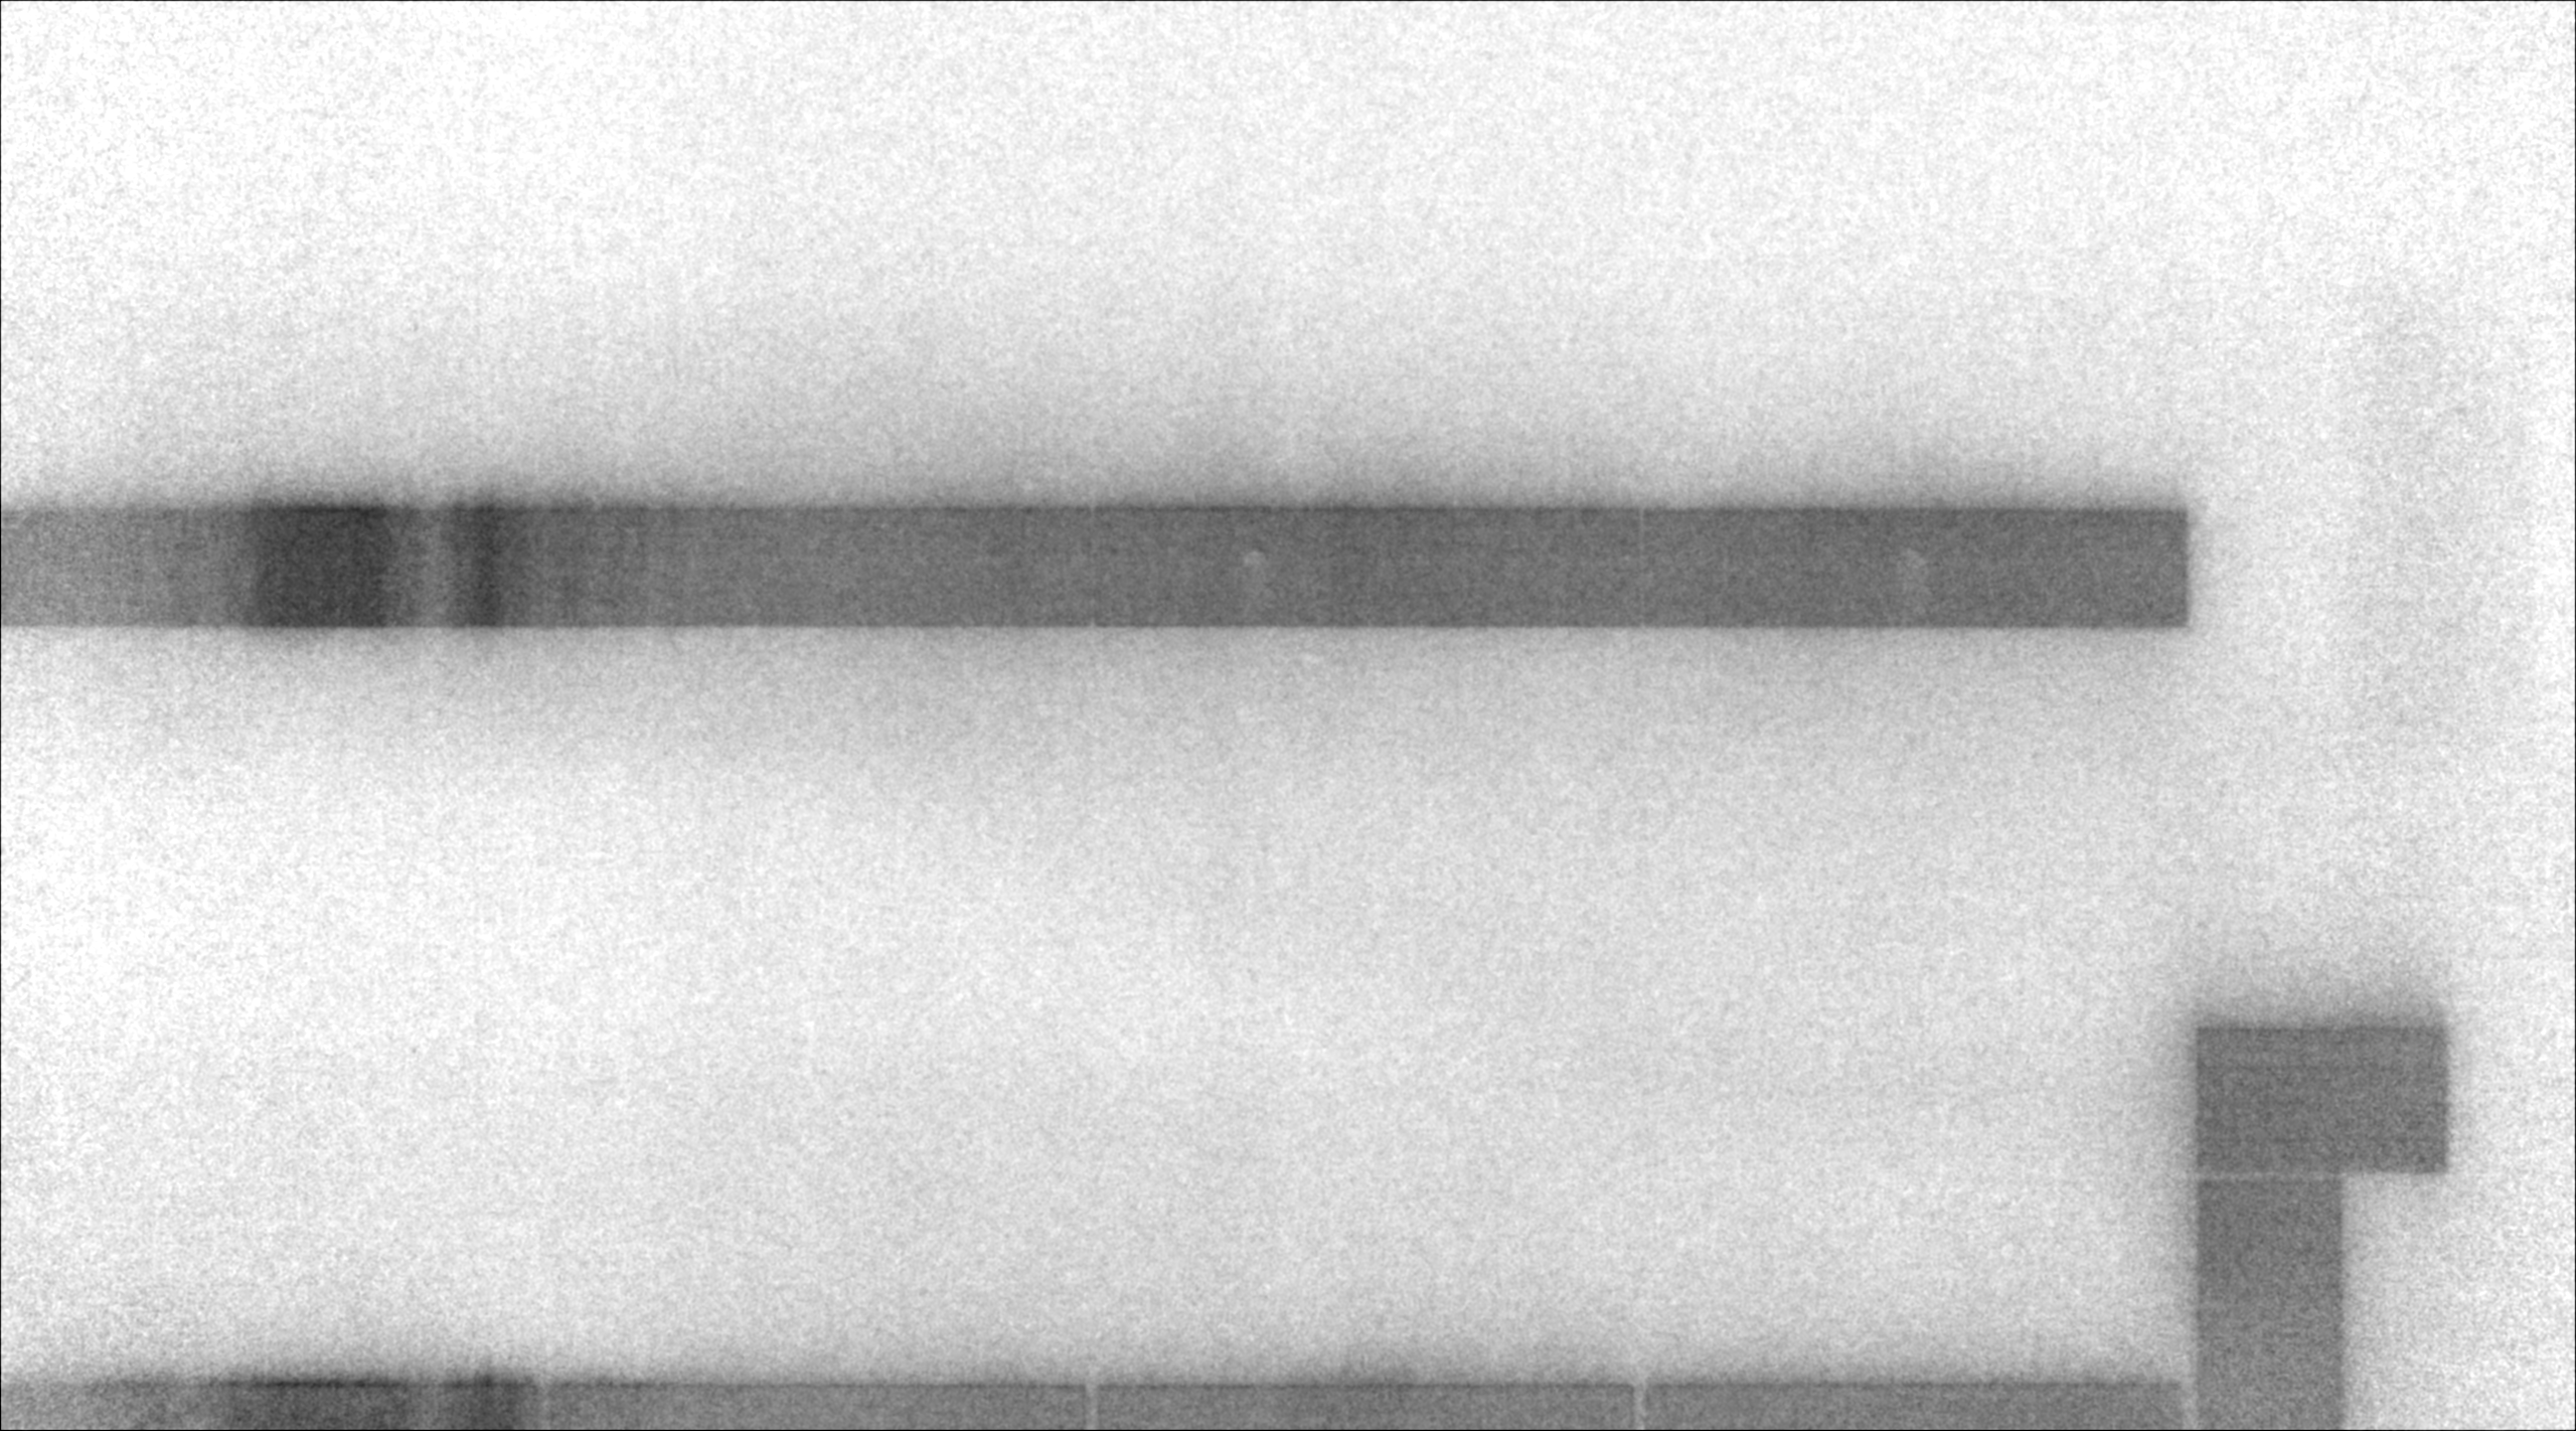
\includegraphics[width=\textwidth]{images/layer_dark_scratch}
    \caption{Layer with dark spots.}

  \end{subfigure}

  \begin{subfigure}{\textwidth}
    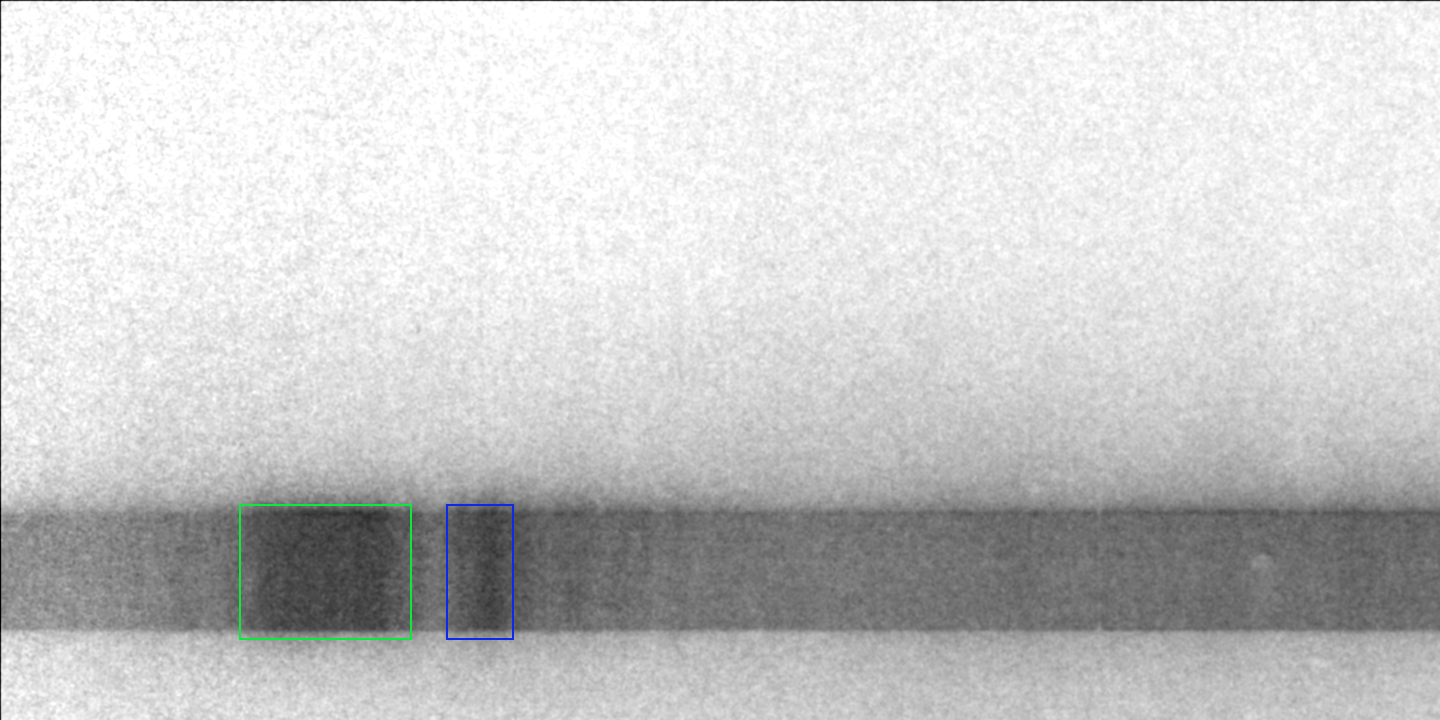
\includegraphics[width=\textwidth]{images/layer_dark_scratch_cropped}
    \caption{Zoomed to the upper left corner of the layer. The green bounding box is safely a dark spot, but the blue bounding box is an ambiguous case.}
  \end{subfigure}

  \caption{Dark spot or scratch?}
  \label{fig:layer_dark_scratch}


\end{figure}
